\chapter{Other applications and future work}
\label{chap:applications}

Both \mx and \varan are designed as flexible frameworks which could be extended
to support a variety of application scenarios involving NVX systems. In this
chapter, we discuss four such scenarios: regression testing
(\S\ref{sec:testing}), live sanitization (\S\ref{sec:sanitization}),
record-replay (\S\ref{sec:record_replay}), and security honeypots
(\S\ref{sec:honeypot}). We also present other possible future extensions to
both \mx and \varan.

% \subsubsection{Regression Testing}
% \label{sec:testing}

% One of the most obvious applications of \varan framework is regression testing.
% Developers often made various assumption about their programs. When working on
% a new version, regression testing is often used to ensure that these
% assumptions still hold even in the new version. Unfortunately, testing is not
% an exhaustive technique and since regression tests are often written by the
% same developers as the software itself, there is a high probability that some
% violations will be violated leading to security bugs~\todo{Give concrete
% examples.}.

% Executing the regression suite under \varan while running both versions in
% parallel (possibly even more) might help to reveal the subtle differences,
% otherwise undetected by the tests. Our current prototype can be instructed to
% stop the application when a divergence in the event stream is discovered
% providing a detailed information of the difference (\eg system call and its
% arguments). \varan may also attempt to continue execution performing different
% system calls. However, this may not always be possible (\eg in case of network
% communication), see discussion in \ref{sec:patternmatching} for more details.

\section{Regression testing}
\label{sec:testing}

By default, whenever \mx detects a divergence between the two versions which
are being run in parallel, it either discard one of the versions, or, if the
divergence is caused by the segmentation fault, it tries to recover the failing
version (\S\ref{sec:rem}). This mode of operation is suitable as a way for
improving reliability of updated software, as shown in
Section~\ref{sec:reliability-evaluation}.

However, \mx can be also used in a different mode, in which the application is
fail-stopped whenever a divergence is detected. This mode of operation is
suitable for regression testing. When working on the new version of the
application developers would typically use the regression suite to ensure that
the new version does not break the existing functionality. When such a situation
occurs, the first step is typically to determine where the bug was introduced.
While this may be easy for simple sequential applications, such task could be
challenging for applications which use non-deterministic inputs such as network
events or random number generators.

One of the main goals of \mx is to intercept all sources of non-determinism and
provide both versions with the same input. This allows developers to run both
versions in parallel, and see whether the patch introduces any divergence by
running both applications in lockstep. When a divergence is detected, \mx can
also provide developers with additional information such as the stack trace
obtained by the \rem component.

While conceptually simple, we believe this mechanism could be helpful in many
development scenarios. Furthermore, we believe it could be integrated with
other mechanisms such as \lstinline`git bisect`, which normally relies on the
regression testing suite, which might be too coarse grained in some scenarios,
but when combined with \mx it can also detect more subtle differences (\eg due
to non-determinism).

\section{Live sanitisation}
\label{sec:sanitization}

\begin{figure}[t]
  \begin{center}
    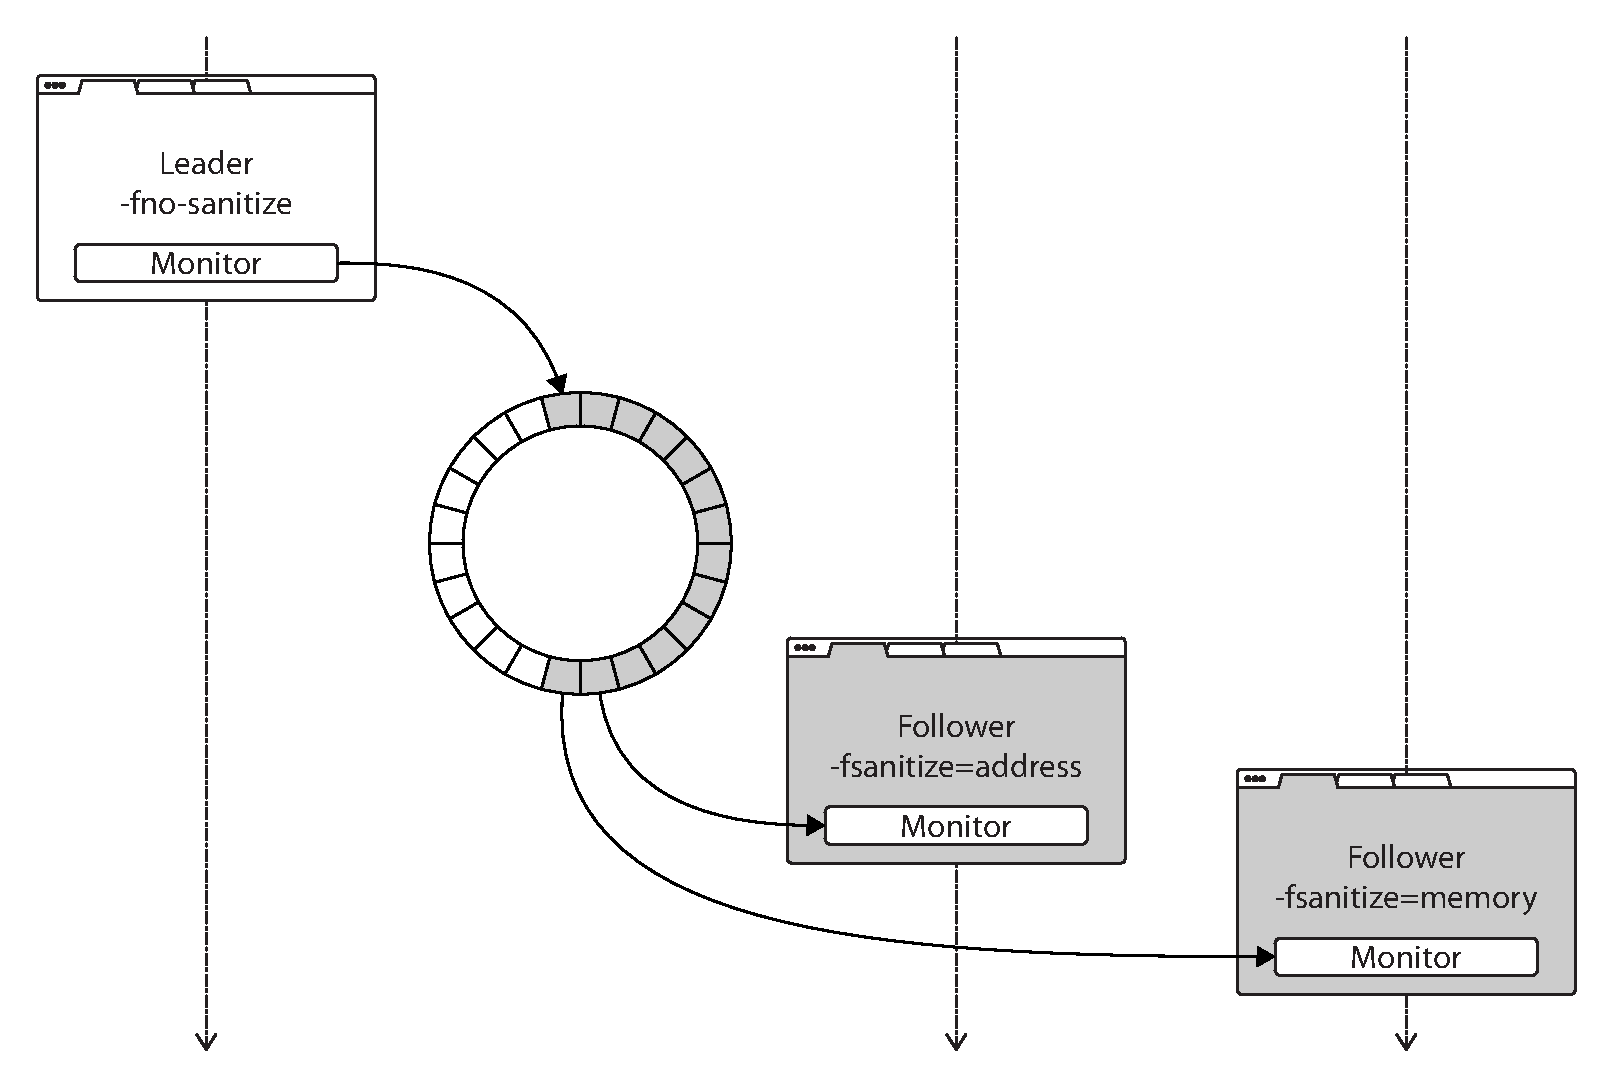
\includegraphics[width=0.75\columnwidth]{applications/figures/live-sanitization}
    \caption{The use of event-streaming architecture for live sanitisation.}
    \label{fig:live-sanitization}
  \end{center}
\end{figure}

Sanitisation is one of the most effective testing techniques for revealing
low-level bugs such as uninitialised pointer dereferences and use-after-free
errors.  Both Clang and GNU C Compiler now include a set of
sanitisers---AddressSanitizer (ASan), MemorySanitizer (MSan), ThreadSanitizer
(TSan)---which can be used to statically instrument the code with various
checks.  Unfortunately, these checks introduce extra overhead (\eg $~2\times$
for ASan, $~3\times$ for MSan and $~5$-$15\times$ for TSan).  which is why
these sanitisers are typically only used in an offline testing. However, during
testing developers only use a limited set of inputs which might not reveal all
bugs.

One possible solution is to record execution traces during deployment and then
replay them in a testing environment with sanitisation enabled. However, this
approach is unlikely to work in practice for several reasons. First, since we
do not know in advance which traces are potentially interesting (\eg trigger
sanitisation checks) and which are not, we have to potentially collect and
replay a huge number of execution traces. Even with some form of deduplication,
this is usually impractical. Second, for long-running applications such as
servers, the log size will quickly grow to a large size. Third, many customers
will refuse to share the logs from their production deployment.

With \varan, we can perform live sanitisation by running the native unsanitised
version as the leader, with sanitised versions as followers, as shown in
Figure~\ref{fig:live-sanitization}.  While sanitisation itself introduces a
performance overhead, since followers do not need to execute any I/O operations
and merely replay them, they can often keep up with the leader, allowing users
to run sanitised versions in production without introducing any significant
overhead.

To demonstrate this, we build revision \lstinline`7f77235` of \redis twice:
once using Clang without any sanitisation, once with ASan enabled.  We then ran
both versions in parallel using \varan and used the same benchmark with the
same settings as for our performance evaluation (\S\ref{sec:c10k}). As
expected, we have not measured any additional slowdown in the leader compared
to the scenario with two non-sanitised versions being run in parallel. To get a
better insight into the effect of running the sanitised version with \varan, we
have measured the median length of the log, \ie the distance between the leader
and the follower. With sanitisation, this length increases from
\redisNoSanitizationMedianLength to \redisSanitizationMedianLength, which does
not impose any problems.

\section{Record-replay}
\label{sec:record_replay}

Although \varan shares similarities with record-replay systems, there are
significant differences; in particular, the log is of fixed size and
only kept in-memory.  However, it is possible to easily extend \varan to
provide full record-replay capabilities by implementing two artificial
clients:
\begin{inparaenum}[(i)]
\item one acting as a \emph{follower} whose only goal is to write the
  content of the ring buffer to persistent storage, and
\item one acting as a \emph{leader}, reading the content of the log
  from the persistent storage and publishing events into the ring
  buffer for consumption by other clients.
\end{inparaenum}

Compared to some of the previous record-replay systems, \varan has a
number of advantages. First, decoupling the logic responsible for
reading/writing the log from the actual application into a separate
process allows the application to run at nearly full speed and utilize
the multiple cores available in modern CPUs.  Second, since \varan was
designed to run multiple instances at the same time, we can replay
multiple versions at once, \eg to determine which versions of the
application from a given range are susceptible to a crash reported by
the user.

We have implemented a simple prototype of the two aforementioned
clients on top of \varan and compared its performance against
\scribe~\cite{scribe}, a state-of-the-art record-replay system
implemented in the kernel.  Unfortunately, because \scribe is
implemented in the kernel and is only maintained for an old 32-bit
Linux kernel (2.6.35), we had to run our experiments inside a virtual
machine (kindly provided to us by \scribe's authors, as the source tree
was broken at the time of our experiments). 
%% This experience clearly shows one of the main disadvantages of
%% kernel-level frameworks---the difficulty of maintaining the code base.
To allow for a more faithful comparison, we ran \varan inside the same
virtual machine.

We used \redis as a benchmark, running the same workload as before,
and configured both systems to record the execution to persistent
storage.  We recorded an overhead of \redisRROvhScribe for
\scribe,\footnote{The overhead we measured for \scribe is higher than
  the overhead reported in~\cite{scribe}; however, note that the original
  work used less aggressive benchmarks such as \httpd.  The use of a
  virtual machine also affected the result.}  compared to
\redisRROvhNx for \varan.
%(but remember that we ran it inside a virtual machine)

% Despite being implemented in the kernel, \scribe
% performed worse than \varan on our \redis experiments: the overhead
% introduced by \scribe was \redisRROvhScribe, compared to only
% \redisRROvhNx for \varan.



\section{Security honeypot}
\label{sec:honeypot}

The ability to perform parallel multi-version execution could be also used to
deploy high-interaction honeypots that can offer a detailed account of the
attackers' activities. These honeypots could run vulnerable versions of
security critical services, and compare their behaviour, in real time, against
that of a known secure version.  Any divergence detected could be resolved in
favour of the secure version and logged for further analysis.  This would
provide a fine-grained understanding of the anatomy of an attack, which is
typically not possible with today's honeypot deployments. The construction of
such a honeypot system using an existing multi-variant execution environment
has been already proposed in the past~\cite{jackson10} but, to our knowledge,
no implementation of such mechanism exists.
%The use of multi-variant execution to construct such honeypot systems has been
%already proposed in the past~\cite{jackson10}. However, to our knowledge, no
%general-purpose implementation of such mechanism exists.

We have implemented this security mechanism in a simple prototype system based
on top of \varan~\cite{pes:mvh}. This system runs two variants of an
application---\emph{public} and \emph{private}---in lockstep and monitors their
behavior. A monitor synchronises the execution of the two variants and grants
or denies access to operating system resources. Any divergence in the variant
behavior might be a sign of an ongoing attack. While this prototype reuses a
large part of the \varan's codebase, namely the preloader, the monitor and the
system call interception mechanism, there are several important differences.

In a regular multi-variant or multi-version application, all versions run on
the same machine under the same security restrictions.  However, in the
honeypot system, each variant has a different access to operating system
resources such as file system and network.

For example, consider a web service running on top of the multi-variant
honeypot (MVH). A public variant is granted access to network resources while
the private variant can only access the file system. Every request received by
the public variant is forwarded to the private variant through the monitor, and
after being processed, the result is sent back to the public version. When the
public version is compromised due to an existing (potentially unknown)
vulnerability, it might issue an additional system call in an attempt to
access local resources; this will result in a divergence which will be detected
and recorded by the monitor. The monitor will also close the connection to the
private variant to protect any critical resources.

An altenative approach has been used in the past to implement shadow
honeypots~\cite{shadow-honeypots}, where both the vulnerable and secure version
share the same process and address space and the runtime monitor switches
between the two versions depending on the request. This approach can reduce the
resource usage, but significantly increases the potential attack surface
thereby reducing the security compared to our solution where both versions are
stricly isolated.

\begin{figure}[t]
  \begin{center}
    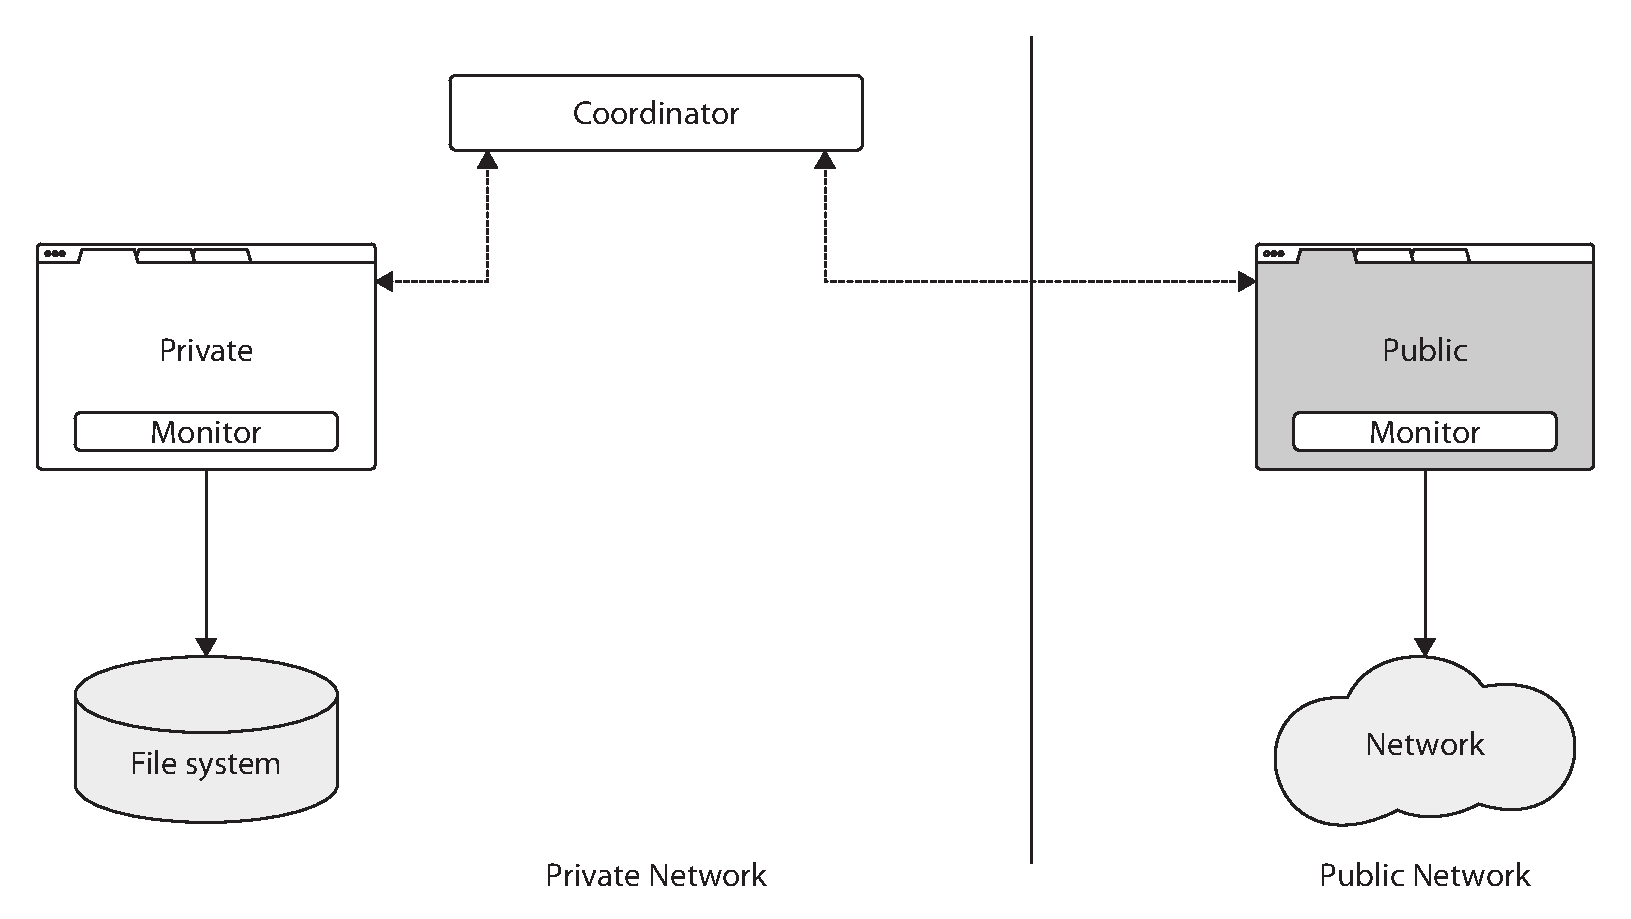
\includegraphics[width=0.75\columnwidth]{applications/figures/honeypot}
    \caption{The architecture of the multi-variant honeypot system.}
    \label{fig:security-honeypot}
  \end{center}
\end{figure}

The architecture of our prototype system is depicted in
Figure~\ref{fig:security-honeypot}.  To enforce strong separation, each variant
can be run on a different machine. Even if attackers manage to subvert our
monitoring infrastructure and gain full access to the operating system, the
impact of such an intrusion can be minimal as the machine which runs the public
version would not contain any critical resources and would ideally be running
inside a demilitarised zone (DMZ) to prevent access to other machines on the
network.  Such an architecture, however, precludes the use of the shared ring
buffer and the event streaming (\S\ref{sec:streaming}). Instead, in our
prototype, we use network sockets to transfer events between variants and the
monitor. This has a negative impact on the performance; we have observed a
per-system call overhead of \numrange{18}{25}$\times$ in our microbenchmarks.
However, we believe that in the case of honeypot systems, performance overhead
is not the most important factor, as the applications running on top of such
systems are not expected to be used in performance critical scenarios.

We have tested our prototype by running two variants of \lighttpdgen 1.4.28 on
top of our honeypot system, where the private variant has been compiled with
all the security mechanisms provided by GCC enabled, while the public variant
did not use any of these.
%\footnote{We used \lstinline`-fstack-protector-all -Wstack-protector --param
%ssp-buffer-size=4 -pie -PIE -ftrapv -D_FORTIFY_SOURCE=2 -z relro,now` GCC
%options for the private variant and \lstinline`-fno-stack-protector -z
%execstack` options for the public variant.}
We then used an existing exploit~\cite{erickson:hacking-networking} to attack the public variant and
inject shellcode\footnote{\url{http://www.shell-storm.org/shellcode/files/shellcode-658.php}}
which tries to add a root user with a custom password to the system. This
attack has been successfully detected and prevented by the honeypot monitor.

\input{applications/future}
